\begin{surferPage}[七次曲面]{對稱七次曲面}
這個像星星一樣的曲面是個 $7$ 次曲面。它的奇異點數 $84$ 一直以來都是已知最大的奇異點數。直到2004年,奧利弗·萊布斯(Oliver Labs)將最大奇異點數提高到 $99$。
從圖中觀察到的三個墊子是由切比雪夫多項式(Chebychev polynomial)導致的,這與霍穆托夫(Chmutov)八次曲面類似。實際上,這個星形曲面是霍穆托夫曲面的一個變形。對某個適當選取的 $\lambda\in\RR$,這裡平面曲線 $S_7(xy):$
\[S_7(x,y) + \lambda \cdot T_d(z) = 0,\]
$T_d(x)+T_d(y)$ 被一個正 $7$ 邊形所替代。
\vspace*{-0.3em}
    \begin{center}
      \begin{tabular}{c@{\qquad}c}
        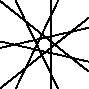
\includegraphics[height=1.5cm]{labsseptic1.pdf}
        &
        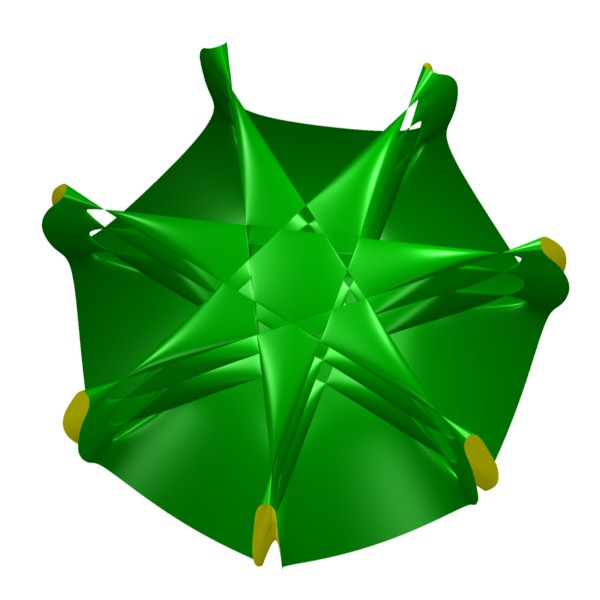
\includegraphics[height=1.5cm]{septic_7eck_von_oben}
      \end{tabular}
    \end{center}
    \vspace*{-0.3em}
這個霍穆托夫構造的變形是由杜克·范·斯特芬(Duco van Straten)提供的。
\end{surferPage}
